\chapter{Wcześniejsze rozwiązania}\label{r:losers}

% TODO: dlaczego nasze rozwiązanie jest najlepsze
Dotychczasowe rozwiązania problemu przeszukiwania bazy tabliczek opierają się o formularze, na podstawie których można zdefiniować jakich tabliczek szukamy. Różnią się one przede wszystkim poziomem skomplikowania formularzy a tym samym ilością parametrów na podstawie których można wyszukiwać tabliczki. Podstawową wadą takich rozwiązań jest brak możliwości tworzenia zapytań złożonych i brak elastyczności.

% W chwili obecnej nie istnieje język dostosowany do potrzeb sumerologów. Jedyne znane nam rozwiązania przedstawionego wyżej problemu opierają się o pomysł formularzy, które w łatwy sposób można wypełniać i łatwo na ich podstawie tworzyć zapytania. Wadą takich rozwiązań jest brak możliwości tworzenia skomplikowanych zapytań.
Poniżej przedstawimy dwie przykładowe strony internetowe oferujące wyszukiwanie za pomocą formularzy.
\section{The Cuneiform Digital Library Initiative \cite{cdli}}
\begin{figure}[h]
 \centering
 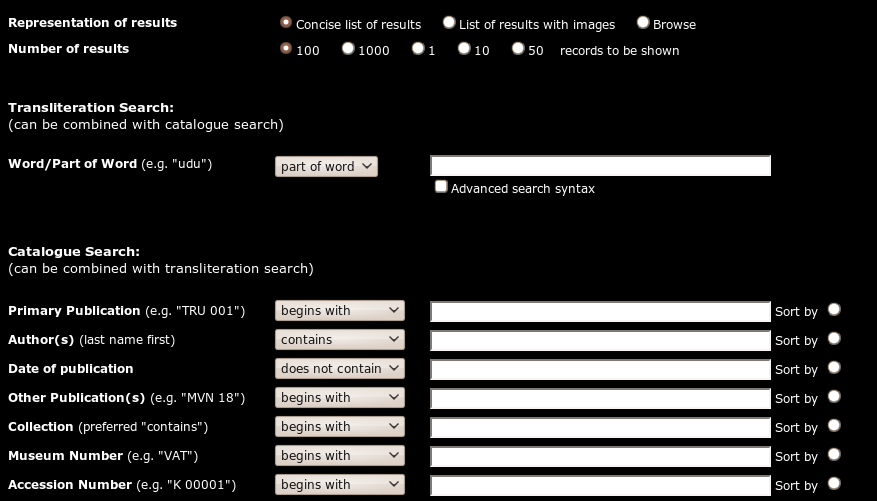
\includegraphics[width=300px]{../diagramy/cdli-search.png}
 % cdli-search.png: 877x501 pixel, 72dpi, 30.94x17.67 cm, bb=0 0 877 501
 \caption{Formularz wyszukiwania na stronie CDLI}
 \label{fig:cdli-search}
\end{figure}
Największą znaną nam bazą tekstów sumeryjskich jest The Cuneiform Digital Library Initiative (CDLI), która zawiera ok 225 tys. tabliczek. Posiada stosunkowo rozbudowany formularz, pozwala na wyszukiwanie po wielu parametrach tabliczki (m. in. dane dot. czasu i miejsca powstania, komentarze CDLI). Dla każdego parametru jest pole tekstowe z możliwymi opcjami wyszukiwania: ``begins with``, ``contains'', ''does not contain''. Dla treści jest pole tekstowe z opcjami ``word``, ``part of word``. Jest również checkbox ''advanced search syntax'', jednak brakuje wyjaśnienia jak go używać.
Nie można tworzyć bardziej skomplikowanych warunków (np. nie można wyszukać tabliczek, które powstały w Uruk lub w Garshanie) ani zapytań złożonych.

% CDLI to największa znana nam baza tekstów sumeryjskich, zawiera ok. 225 tys. tekstów. 
% Umożliwia wyszukiwanie po wielu parametrach.
% Dla każdej metadanej jest pole tekstowe z możliwymi opcjami wyszukiwania: ``begins with``, ``contains'', ''does not contain''. 
% Dla treści jest pole tekstowe z opcjami ``word``, ``part of word``.
% Jest również checkbox ''advanced search syntax'', jednak brakuje wyjaśnienia jak go używać.
% Nie można tworzyć bardziej skomplikowanych warunków dla poszczególnych parametrów oraz zapytań złożonych.

\section{The Electronic Text Corpus of Sumerian Literature \cite{etcsl}} 
\begin{figure}[h]
 \centering
 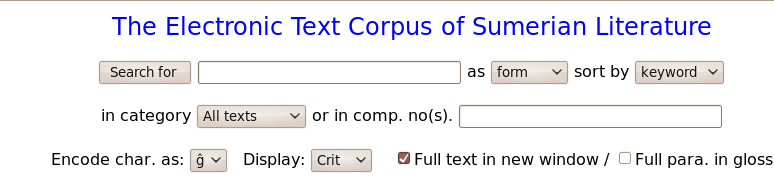
\includegraphics[width=300px]{../diagramy/etcsl-search.png}
 % etcsl-search.png: 774x182 pixel, 72dpi, 27.31x6.42 cm, bb=0 0 774 182
 \caption{Formularz wyszukiwania na stronie ETCSL}
 \label{fig:etcsl-search}
\end{figure}

The Electronic Text Corpus of Sumerian Literature posiada znacznie mniejszą bazę, zawierającą głównie teksty literackie. 
Ma ograniczone możliwości wyszukiwania po metadanych (tylko po kategorii tekstu), jednak udostępnia tworzenie bardziej 
skomplikowanych zapytań dotyczących treści tabliczki. 
Pozwala określić typ wyszukiwanego słowa (form, lemma, label, pos, emesal, sign),
 a także jego znaczenie w tekście (np. czy jest imieniem bóstwa) oraz część mowy, do której należy. 
Można również wyszukiwać po fragmencie słowa.
